\section{Modeling first stage problem}

We propose a 1D quasi-steady approximation of the combustion problem
using the approximations from Section~\ref{sec:assumptions}. Note
that, although the conservation laws are strict inequalities,
they have been relaxed to be modeled in a difference-of-convex
optimization framework.

\subsection{Geometric explanation}

\tdplotsetmaincoords{50}{130}
\tdplotsetrotatedcoords{0}{90}{0}
\begin{tikzpicture}[tdplot_main_coords]
    \draw[thick,->] (0,0,0) -- (1,0,0) node[anchor=north east]{$l$};
    \draw[thick,->] (0,0,0) -- (0,1,0) node[anchor=north west]{$r$};
    \tdplotdrawarc[tdplot_rotated_coords, color=blue]{(0,0,-4)}{2}{0}{360}{anchor=north west}{$\pi r^2$};
    \tdplotdrawarc[tdplot_rotated_coords, color=blue]{(0,0,0)}{2}{0}{360}{anchor=north west}{$\pi r^2$};

    \tdplotsetcoord{P}{1.5}{0}{0}
    \tdplotsetcoord{B}{1.5}{45}{0}
    draw[-stealth, color=red]

\end{tikzpicture}

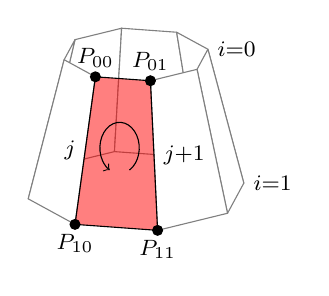
\begin{tikzpicture}[join=round]
    \tikzstyle{conefill} = [fill=blue!20,fill opacity=0.8]
    \tikzstyle{ann} = [fill=white,font=\footnotesize,inner sep=1pt]
    \tikzstyle{ghostfill} = [fill=white]
    \tikzstyle{ghostdraw} = [draw=black!50]


    % Second version of the cone

\begin{scope}[xshift=3.5cm]
    \filldraw[ghostdraw,ghostfill](-.775,1.922)--(-1.162,.283)--(-.274,.5)
                                   --(-.183,2.067)--cycle;
    \filldraw[ghostdraw,ghostfill](-.183,2.067)--(-.274,.5)--(.775,.424)
                                   --(.516,2.016)--cycle;
    \filldraw[ghostdraw,ghostfill](.516,2.016)--(.775,.424)--(1.369,.1)
                                   --(.913,1.8)--cycle;
    \filldraw[ghostdraw,ghostfill](-.913,1.667)--(-1.369,-.1)--(-1.162,.283)
                                   --(-.775,1.922)--cycle;
    \filldraw[ghostdraw,ghostfill](.913,1.8)--(1.369,.1)--(1.162,-.283)
                                   --(.775,1.545)--cycle;
    \filldraw[ghostdraw,ghostfill](-.516,1.45)--(-.775,-.424)--(-1.369,-.1)
                                   --(-.913,1.667)--cycle;
    \filldraw[ghostdraw,ghostfill](.775,1.545)--(1.162,-.283)--(.274,-.5)
                                   --(.183,1.4)--cycle;
    \filldraw[fill=red,fill opacity=0.5](-.516,1.45)--(-.775,-.424)--(.274,-.5)
                                         --(.183,1.4)--cycle;
    \fill(-.775,-.424) circle (2pt);
    \fill(.274,-.5) circle (2pt);
    \fill(-.516,1.45) circle (2pt);
    \fill(.183,1.4) circle (2pt);
    \path[font=\footnotesize]
            (.913,1.8) node[right] {$i\hbox{$=$}0$}
            (1.369,.1) node[right] {$i\hbox{$=$}1$};
    \path[font=\footnotesize]
            (-.645,.513) node[left] {$j$}
            (.228,.45) node[right] {$j\hbox{$+$}1$};
    \draw (-.209,.482)+(-60:.25) [yscale=1.3,->] arc(-60:240:.25);
    \fill[black,font=\footnotesize]
                    (-.516,1.45) node [above] {$P_{00}$}
                    (-.775,-.424) node [below] {$P_{10}$}
                    (.183,1.4) node [above] {$P_{01}$}
                    (.274,-.5) node [below] {$P_{11}$};
    \end{scope}
\end{tikzpicture}

\subsection{Constraints}

\subsubsection{Geometric constraints}

We assume that the rocket is divided into $n$ equal sections

\begin{equation}
    \rm{n} \times l_{\rm{sec}} = l
\end{equation}

\subsubsection{Bounding constraints}

We limit the expansion ratio within a single section with parameter $k_{A, \rm{max}}$.

\begin{align}
    k_A &\leq k_{A,\rm{max}} \\
    k_A &\geq \frac{1}{k_{A,\rm{max}}}
\end{align}

\subsubsection{Exit quantities}

To be able to couple a rocket nozzle to the SRM model,
we need to define the SRM exit quantities.

\begin{align}
    u_{\rm{out}} &= u_{\rm{n}-1} \\
    T_{t,\rm{out}} &= T_{t,\rm{n}-1} \\
    T_{\rm{out}} &= T_{\rm{n}-1} \\
    \dot{m}_{\rm{out}} &= \dot{m}_{\rm{n}-1} \\
    \rho_{\rm{out}} &= \rho_{\rm{n}-1} \\
    P_{\rm{out}} &= P_{\rm{n}-1}
\end{align}

\subsubsection{In-cell constraints}

Firstly, we define some simple internal geometry for each section, which are the
chamber volume, area ratio, average area and burn area.

Note that the last constraint, which equates the total internal area to the
sum of the average bore area and the propellant cross-sectional area,
is where the only signomial equality exists.

\begin{align}
    V_{\rm{chamb}, \rm{i}} &= A_{\rm{avg}, \rm{i}} l_{\rm{sec}, \rm{i}} \\
    k_{A, \rm{i}} &= \frac{A_{\rm{in}, \rm{i}}}{A_{\rm{out}, \rm{i}}}  \\
    A_{\rm{avg, i}} &= A_{\rm{in}, \rm{i}} A_{\rm{out}, \rm{i}} \\
    A_{\rm{b, i}} &= l_{\rm{b,i}} l_{\rm{sec}} \\
    \pi r^2 &= A_{\rm{avg, i}} + A_{\rm{p, in, i}}
\end{align}

There are some constraints on the geometry of the cross-section, which we define
as the burn area $A_{\rm{b}}$ and burn length $l_{\rm{b}}$. Firstly, since the most efficient
shape w.r.t. burn length vs. area is a circle, the burn length has to be greater than the smallest possible circle
with the same average area as the bore of the rocket. On the other hand, we also want to
upper bound the geometry so the burn cross-sectional length cannot be greater than some factor
$l_{\rm{b,max}}$ times the circumference of that circle.

\begin{align}
    l_{\rm{b}} &\geq 2 \sqrt{\pi A_{\rm{avg, i}}} \\
    l_{\rm{b}} &\leq l_{\rm{b,max}} \times 2 \sqrt{\pi A_{\rm{avg, i}}}
\end{align}

The chamber pressure $P_{\rm{chamb}, \rm{i}}$ is defined as the geometric average of
the inlet and outlet static pressures. We assume ideal gas, which is a poor assumption,
but is deemed satisfactory for a conceptual analysis.

\begin{align}
    P_{\rm{chamb}, \rm{i}}^2 &= P_{\rm{i}-1} P_{\rm{i}} \\
    P_{\rm{i}} = \rho_{\rm{i}} R T_{\rm{i}} \\
\end{align}

The burn rate in a given cell $\rm{i}$ is defined by the following inequality,
which is an empirical relation of the burn rate to chamber static
pressure and local flow velocity:

\begin{equation}
r_{\rm{i}} \geq r_c  \Big(\frac{P_{chamb,\rm{i}}}{\hat{P}}\Big)^{0.35} (1 + \frac{1}{2} r_k (u_{\rm{i}-1} + u_{\rm{i}}))
\end{equation}

where $r_c$ is a burn rate coefficient, $\hat{P}$ is a and $r_k$ is a non-dimensionalized parameter
which describes the rate of erosive burning. These coefficients
depend on the propellant used, but for this model are set at
$5.6~\rm{mm/s}$, $10^{6}~\rm{Pa}$, and $0.05~\rm{1/(m/s)}$ respectively. Using burn rate $r$,
we also bound the amount of fuel remaining after every time step.

\begin{equation}
    A_{\rm{p, out, i}} + r_{\rm{i}} l_{\rm{b, i}} \Delta t \leq A_{\rm{p, in, i}}
\end{equation}

Mass flow rate is the product of density, velocity and cross-sectional area.
Product generation rate $q$ is related to the propellant density $\rho_{\rm{p}}$,
burn rate $A_{\rm{b}}$, and burn rate $r$.

\begin{align}
    \dot{m}_{\rm{i}} &= \rho_{\rm{i}} u_{\rm{i}} A_{\rm{out}, \rm{i}} \\
    q_{\rm{i}} &= \rho_{\rm{p}} A_{\rm{b, i}} r_{\rm{i}} \\
\end{align}

And of course, for the basic fluid dynamic analysis, we define the total temperature
and don't allow for the internal flow to go supersonic.

\begin{align}
    T_{\rm{t,i}} &\leq T_{\rm{i}} + \frac{u_{\rm{i}}^2}{2c_{p}} \\
    u_{\rm{i}}^2 &\leq \rho_{\rm{i}} R T_{\rm{i}}
\end{align}

\subsubsection{Cell coupling/conservation constraints}

The inlet area of one cell is the outlet area of another

\begin{equation}
    A_{\rm{in}, \rm{i}} = A_{\rm{out}, \rm{i}-1}
\end{equation}

The static pressure in previous cell $\rm{i}-1$ must be strictly higher
than in cell $\rm{i}$, since the flow must be toward the nozzle.

\begin{equation}
    P_{\rm{i}-1} \geq P_{\rm{i}}
\end{equation}

The different conservation laws are as follows:

\begin{align}
    \dot{m}_{\rm{i}-1} + q_{\rm{i}}
    &\geq
    \dot{m}_{\rm{i}} &\rm{[Mass Cons.]}\\
    P_{\rm{i}-1} A_{\rm{in}, \rm{i}} + \rho_{\rm{i}-1} u_{\rm{i}-1}^2 A_{\rm{in},\rm{i}}
    &\geq
    P_{\rm{i}} A_{\rm{out}, \rm{i}} + q_{\rm{i}} u_{\rm{i}} V_{\rm{chamb},\rm{i}} l_{\rm{sec}} A_{\rm{out},\rm{i}}
    + \rho_{\rm{i}-1} u_{\rm{i}-1} u_{\rm{i}} A_{\rm{out}, \rm{i}}&[\mathrm{Mom. Cons.}] \\
    \dot{m}_{\rm{i}-1} T_{t, \rm{i}-1} + q_{\rm{i}}\Big(T_{\rm{amb}} + \frac{k_{\rm{comb}}}{c_{\rm{p}}}\Big)
    &\geq
    \dot{m_{\rm{i}}} T_{t, \rm{i}} &\rm{[Energy Cons.]} \\
\end{align}

\subsubsection{First cell constraints}

We define \textit{the first cell} as the first gas-generating section
of the rocket, i.e. the one that has no incoming flow.
Since there is no influx of mass, momentum or energy into that cell,
the conservation laws are simplified.
The pressure drop in the first section is the $\delta P$ required
to accelerate the mass flow in the first section. The mass flow out of
the first section is simply the mass generated in that section.

\begin{align}
    \dot{m}_0 &= q_0 &\mathrm{[Mass Cons.]} \\
    P_{end}*A_{\rm{in}, 0} &\geq P_0 A_{\rm{out}, 0} + q_0 u_0 V_{\rm{chamb},0} l_{\rm{sec}} A_{\rm{out},0} &\mathrm{[Mom. Cons.]} \\
    T_{t, 0} \dot{m}_0 &\leq q_0 (T_{\rm{amb}} + k_{comb,p} c_{p}) &\mathrm{[Energy Cons.]}
\end{align}

We also define $P_{\rm{end}}$, which is the pressure at the tip of the rocket where there is stagnation.
Since there is no influx to the first section, the burn rate constraint is simplified.

\begin{align}
    P_{\rm{chamb}, 0}^2 &= P_{\rm{end}} P_0 \\
    r_{0} \geq r_c  \Big(\frac{P_{\rm{chamb},0}}{\hat{P}}\Big)^{0.35} (1 + \frac{1}{2} r_k (u_{0}))
\end{align}

\subsubsection{Nozzle constraints}

The nozzle chokes the flow, and given some ambient pressure,
produces thrust through a combination of mass ejection and
pressure differential



	% --------------------------------------------------------------
	%     You don't have to mess with anything below this line.
	% --------------------------------------------------------------

% Previous attempts

%	The hope is that the problem can be posed as a difference-of-convex optimization problem, and especially a mixed integer convex problem through piecewise linearization and the use of binary variables.
%	The pipe dream is to be able to perform this optimization in 3D with good first-order methods to accommodate for erosive burning.


%	\subsection{Alternative ways to think about the burn rate}
%	We can also think about the burn rate being faster in regions that are more exposed to the flame (thinking about the dot product of the two vectors originating from the point), and then assigning a binary value on whether or not the resulting vector is within or outside of the burning surface depending on the cross product of the two vectors. However, this is more easily said than done, since both of these vector operations are non-convex.
%

%		\section{Preliminary Optimization Problem}
%
%	To test whether or not the method of vector translations can be solved
%	in a mixed integer convex form, we formulate the following problem
%
%	\subsection{Parameters}
%	\begin{itemize}
%	\item \textbf{$n_{ctrl}$:} number of control points
%	\item \textbf{$n_t$:} number of time steps
%	\item \textbf{$r$:} radius of the rocket
%	\item \textbf{$R$:} regression rate of fuel
%	\item \textbf{$C_{profile}$:} burn surface length desired (vector of $n_t$)
%	\end{itemize}
%
%	\subsection{Variables}
%	\begin{itemize}
%		\item \textbf{$x_{i,t}$:} x-dimension of the control point i at time t
%		\item \textbf{$\Delta x_{i,t}$:} vector from point $x_{i-1,t}$ to $x_{i,t}$.
%		\item \textbf{$y_{i,t}$:} y-dimension of the control point i at time t
%		\item \textbf{$\Delta y_{i,t}$:} vector from point $y_{i-1,t}$ to $y_{i,t}$.
%		\item \textbf{$l_{i,t}$:} length of vector from $(x,y)_{i-1,t}$ to $(x,y)_{i,t}$
%		\item \textbf{$C_{t}$:} the length of the burn surface at time t
%		\item \textbf{$n_{x_{i,t}}$:} normal vector of edge to the LHS of node i at time t
%		\item \textbf{$n_{y_{i,t}}$:} normal vector of edge to the LHS of node i at time t
%	\end{itemize}
%
%	\subsection{Untransformed constraints}
%
%	The raw formulation, without any regard for linearity or convexity
%	is as follows:
%
%	\begin{align}
%	& \min &&\sum_{t=1}^{n_t} (C_{t} - C_{profile})^2 \\
%	& \text{ s.t.} && r^2 \geq x_{i,t}^2 + y_{i,t}^2, \forall i, t \label{eq1} \\
%	& && \Delta x_{i,t} = x_{i,t} - x_{i-1,t} \label{eq2}\\
%	& && \Delta y_{i,t} = y_{i,t} - y_{i-1,t} \label{eq3} \\
%	& && l_{i,t}^2 = \Delta x_{i,t}^2 + \Delta y_{i,t}^2 \label{eq4} \\
%	& && C_{t} = \sum\limits_{i=1}^{n_{ctrl}} l_{i,t} \label{eq5} \\
%	& && n_{x_{i,t}} = \frac{-\Delta y_{i,t}}{l_{i,t}} \label{eq6} \\
%	& && n_{y_{i,t}} = \frac{\Delta x_{i,t}}{l_{i,t}} \label{eq7} \\
%	& && x_{i,t+1} = x_{i,t} + \frac{1}{2} R (n_{x_{i,t-1}}+ n_{x_{i+1,t-1}}) \label{eq8} \\
%	& && y_{i,t+1} = y_{i,t} + \frac{1}{2} R (n_{y_{i,t-1}}+ n_{y_{i+1,t-1}}) \label{eq9} \\
%	\end{align}
%
%	\section{Dealing with nonlinearities and nonconvexities}
%	\begin{itemize}
%		\item \textbf{Objective:} Nonlinear but convex. Can leave be.
%		\item \textbf{Equation~\ref{eq1}:} Nonlinear but convex. Can leave be.
%		\item \textbf{Equation~\ref{eq2}:} Linear.
%		\item \textbf{Equation~\ref{eq3}:} Linear.
%		\item \textbf{Equation~\ref{eq4}:} Linear.
%		\item \textbf{Equation~\ref{eq5}:} Since this is an equality it is non-convex. We also want this to be tight. So we insert two auxiliary variables, and do a piecewise linearization of the quadratic terms.
%%	\begin{align}
%%	l_{i,t}^2 = \Delta x_{i,t}^2 + \Delta y_{i,t}^2
%%	\end{align}
%		\item \textbf{Equation~\ref{eq6}:} Linear.
%		\item \textbf{Equation~\ref{eq7}:} Nonlinear, and convexity depends on sign of $\Delta y$.
%		\item \textbf{Equation~\ref{eq8}:} Nonlinear, and convexity depends on sign of $\Delta x$.
%		\item \textbf{Equation~\ref{eq9}:} Linear.
%
%	\end{itemize}
%
%	\section{Modifying Constraints}
%
%	\subsection{Relaxing the Diameter Constraint}
%
%	\subsection{Non GP compatible constraints}
%	The three non GP compatible constraints are:
